\documentclass[11pt]{article}\usepackage[margin=1in]{geometry}\usepackage{amsmath,amssymb,amsthm,mathtools}\usepackage{graphicx}\graphicspath{{figures/}{../figures/}{figs/}{./}}\usepackage{enumitem}\usepackage{hyperref}\usepackage{cleveref}\usepackage{tikz}\usetikzlibrary{arrows.meta,positioning,calc,shapes.geometric}\usepackage{float}\usepackage[most]{tcolorbox}\usepackage{kotex}\usepackage{booktabs}\emergencystretch=1.6em\tolerance=2000 \crefname{assumption}{Assumption}{Assumptions}\Crefname{assumption}{Assumption}{Assumptions}\crefname{definition}{Definition}{Definitions}\Crefname{definition}{Definition}{Definitions}\crefname{proposition}{Proposition}{Propositions}\Crefname{proposition}{Proposition}{Propositions}\crefname{fact}{Fact}{Facts}\Crefname{fact}{Fact}{Facts} \newtheorem{assumption}{Assumption}\newtheorem{definition}{Definition}\newtheorem{lemma}{Lemma}\newtheorem{proposition}{Proposition}\newtheorem{theorem}{Theorem}\newtheorem{corollary}{Corollary}\newtheorem{fact}{Fact}\theoremstyle{remark}\newtheorem{remark}{Remark} \newcommand{\R}{\mathbb{R}}\newcommand{\U}{\mathcal U}
\newcommand{\Cset}{\mathcal C}\newcommand{\Pcl}{\mathcal P}\newcommand{\Zset}{\mathcal Z_0}\newcommand{\Xset}{\mathcal X_0}
\DeclareMathOperator{\clr}{clr}\newcommand{\norm}[1]{\lVert #1\rVert}\newcommand{\what}{\hat w}

\title{적응형 아래층과 양보하는 interface를 가진 RL policy의 학습 비교:\\ 부정적 결과}
\author{Junhyeok Yoon}
\date{2026년 11월 12일}

\begin{document}
\maketitle

\begin{abstract}
사양 문서의 policy 구조가 학습에 이득을 주는지를 2-link arm 과제에서 시험했다. 이 구조에서는 task policy가 의도와 허용 오차를 제안하고, 적응형 아래층이 그 안에서 오차를 지키며, interface가 여유에 따라 양보하고, 아래층이 측정값을 보고한다. 같은 학습 예산에서 입력을 직접 내는 policy에 funnel filter를 붙인 기존 방식이 관절 오차를 가장 작게 만들었고, 그 방식도 관절 제약을 위반하지 않았다. 보고를 관측에서 빼거나 학습된 reflex를 더해도 제안한 구조의 결과는 나아지지 않았다. 명령을 고정해 아래층만 평가해도 오차가 학습된 기존 방식보다 컸으므로, 병목은 학습 신호가 아니라 아래층의 추종이다. 정상 상태 정확도에서는 적응의 이득이 나타난다는 예측을 사전에 등록하고 두 번째 비교를 했으나, 예측은 세 seed 모두에서 틀렸다. 사전에 정한 규칙에 따라 이 설계는 중단한다. 이어서 실패의 원인으로 지목한 네 가지를 사전 등록 후 하나씩 고쳐 보았으나 어느 것도 기준을 넘지 못했고, 모두 함께 고쳐도 기존 방식과의 차이를 절반도 줄이지 못했다. 가장 가까운 선행 연구와의 전문 대조 결과도 적는다.
\end{abstract}

\section{질문}
\label{sec:question}

\textbf{직관 (무엇을 시험하는가).} 제약 노트는 제안한 구조가 모든 weight와 모든 명령에서 관절 제약과 입력 제약을 지킨다는 것을 증명했다. 그 증명은 학습되는 부분의 내용과 무관하므로, 구조가 학습에 무엇을 더하는지는 말하지 않는다. 이 노트는 그것을 두 가설로 나누어 같은 학습 예산에서 시험한다.
\begin{itemize}
\item[\textbf{(H1)}] 제안한 구조는 입력을 직접 내는 policy에 funnel filter를 붙인 구조보다 높은 return을 얻는다.
\item[\textbf{(H2)}] 아래층의 보고를 관측에 넣으면 넣지 않을 때보다 높은 return을 얻는다.
\end{itemize}

\section{Setting}
\label{sec:setting}

\begin{definition}[Task family]
\label{def:task}
\begin{itemize}
\item Plant: a two-link arm in a vertical plane, $M(q)\ddot q+C(q,\dot q)\dot q+g(q)+F_v\dot q=u$, with link masses 4 and 2 kg, link lengths 0.4 m, a tip payload $m_p\sim\mathcal U[0,\bar m_p]$, viscous friction $F_v=\operatorname{diag}(f_1,f_2)$ with $f_i\sim\mathcal U[0.2,1]$, and reflected rotor inertia $\operatorname{diag}(0.3,0.1)$; $m_p$ and $F_v$ are unknown to every controller.
\item Constraints: $q\in\mathcal C_q:=[-0.2,1.2]\times[0.2,1.8]$ rad and $|u_i|\le\bar u_i$.
\item Episode: 3 s from rest at $q(0)$ uniform on $\mathcal C_q$ shrunk by 0.15 rad; target $q^\star_1$ on $[0,1.5)$ s and $q^\star_2$ on $[1.5,3]$ s, each uniform on $\mathcal C_q$ shrunk by 0.03 rad and, with probability $1/2$, moved to 0.03 rad from a randomly chosen joint limit.
\item Reward: $r:=-\norm{q-q^\star}^2-0.01\sum_i(u_i/\bar u_i)^2$, averaged over the episode.
\item Round 1: $\bar m_p=2$ kg, $\bar u=(60,25)$ Nm. Round 2: $\bar m_p=4$ kg, $\bar u=(80,35)$ Nm.
\end{itemize}
\end{definition}

\begin{definition}[Architectures]
\label{def:arch}
Every controller measures $(q,\dot q)$ and $q^\star$, and every policy is a network with two hidden layers of 32 tanh units. With $\eta:=\dot q+2q$:
\begin{itemize}
\item \textbf{\emph{Proposed}}: every 0.05 s the task policy outputs $v_p$ with $\norm{v_p}\le4$ and $\psi_p\in[0.05,0.4]$. The core and the interface are those of the constraint note with $\kappa=15\,\psi_g^2$; fast weights $\hat W$ on 29 fixed random-feature functions $\Phi$ of $(q,\dot q,\dot r_g-2\dot q)$ with $\dot{\hat W}=-10\,\lambda\lambda_{\mathrm{ff}}\,\Phi\,e^\top$ and trained initial value; feedforward bound 40 Nm; $\gamma_r(m)=\gamma_\psi(m)=\min\{1,2m\}$, $\gamma_+(m)=m$, $\alpha=4$, $c_0=0.3$. The observation contains the margins, the saturation factor, the realization gap, the feedback magnitude, the current feedforward and the distance of the fast weights from their initial value.
\item \textbf{\emph{Proposed, no reports}}: identical, with the report entries of the observation set to zero.
\item \textbf{\emph{Proposed, learned reflex}}: the proposed architecture plus a network of $(q,\dot q,q^\star)$, updated every 0.01 s and added inside the feedforward bound; also with the report entries set to zero.
\item \textbf{\emph{Input policy with funnel filter}}: every 0.01 s the policy outputs $u_{\mathrm{RL}}=\bar u\odot\tanh(\cdot)$; with $w_i:=(\eta_i-2c_i)/(2h_i)$, where $c$ and $h$ are the center and the half-widths of $\mathcal C_q$, the input is the direction-preserving saturation of $u_{\mathrm{RL},i}-20\,a_i\,w_i/(1-w_i^2)$, with $a_i$ rising linearly from 0 at $|w_i|=0.8$ to 1 at $|w_i|=0.9$.
\item \textbf{\emph{Input policy with funnel filter and error integral}} (round 2): the observation also contains $\int(q-q^\star)\,dt$ since the last target switch.
\end{itemize}
\end{definition}

\textbf{학습과 평가.} 모든 구조를 같은 evolution strategies로 학습했다. Iteration마다 대칭 쌍 24개의 perturbation을 task 3개에서 평가하고, rank로 정규화한 return으로 Adam step을 둔다(perturbation 크기 0.04, step 0.02). Iteration은 70개이고 run마다 학습 episode는 10,080개이다. Seed는 3개, 평가는 고정된 test task 64개에서 했다. 적분은 4차 Runge--Kutta, 간격 $10^{-3}$초이다.

\textbf{보장의 적용.} 기계 system의 축소에서 속도 상한은 $\bar v/k_1+2\psi_{\max}=2.8$ rad/s이다. 그 영역에서 뽑은 표본 3,000개의 drift 배율 최솟값은 1차 비교의 한계에서 1.346, 2차 비교의 한계에서 1.224이다. 따라서 제약 노트의 방향별 authority 정리가 제안한 구조들에 적용된다.

\section{1차 비교}
\label{sec:round1}

\begin{table}[H]
\centering\footnotesize\setlength{\tabcolsep}{4pt}
\caption{Round 1: final policies on the test tasks}
\label{tab:r1}
\begin{tabular}{p{4.3cm}ccccc}
\toprule
구조 & 관절 오차 [rad] & return & 위반 (학습) & 위반 (test) & 최대 정규화 오차 \\
\midrule
Input policy with funnel filter & 0.289--0.307 & -0.155 & 0 / 30240 & 0 / 192 & 0.908 \\
Proposed & 0.552--0.565 & -0.409 & 0 / 30240 & 0 / 192 & 0.941 \\
Proposed, no reports & 0.540--0.555 & -0.397 & 0 / 30240 & 0 / 192 & 0.941 \\
Proposed, learned reflex & 0.573--0.597 & -0.423 & 0 / 30240 & 0 / 192 & 1.268 \\
Proposed, learned reflex, no reports & 0.517--0.578 & -0.389 & 0 / 30240 & 0 / 192 & 1.380 \\
\bottomrule
\end{tabular}
\end{table}

관절 오차는 seed 3개의 최솟값과 최댓값, return은 평균이다. 최대 정규화 오차는 제안한 구조에서 $\norm{e}/\psi_g$, 입력 policy에서 $\max_i|w_i|$의 학습과 test 전체 최댓값이다. 관절 제약 위반은 다섯 구조 모두에서 없었다. 기존 방식의 관절 오차는 0.289--0.307 rad로 제안한 구조들(0.517--0.597 rad)의 약 절반이다. 보고를 뺀 구조는 뺀 전과 같거나 약간 나았고, 학습된 reflex는 이득을 주지 않았다. 따라서 이 과제와 이 학습 예산에서 (H1)과 (H2)는 모두 지지되지 않는다. 다만 \Cref{fig:rl}(a)에서 제안한 구조들의 오차는 70 iteration에서도 줄고 있었으므로, 학습을 더 하면 차이가 줄어들 수 있다.

\textbf{원인 (명령을 고정한 아래층 평가).} 학습 대신 reference를 목표로 비례 조향하는 명령을 넣어 아래층만 평가했다.
\[
v_p=8\,(2q^\star-r_g)\,\min\Big\{1,\ \frac{\bar v}{8\norm{2q^\star-r_g}}\Big\}.
\]

\begin{table}[H]
\centering\footnotesize
\caption{Lower layer of the proposed architecture under a fixed proportional command}
\label{tab:scripted}
\begin{tabular}{ccccccc}
\toprule
$\bar v$ & $\kappa/\psi_g^2$ & $g_a$ & $\psi_p$ & 관절 오차 [rad] & yield factor 평균 & 최대 $\norm{e}/\psi_g$ \\
\midrule
4 & 15 & 10 & 0.05 & 0.627 & 0.225 & 0.966 \\
4 & 15 & 10 & 0.4 & 0.585 & 0.342 & 0.930 \\
4 & 60 & 10 & 0.05 & 0.556 & 0.365 & 0.931 \\
4 & 60 & 40 & 0.05 & 0.473 & 0.591 & 0.924 \\
6 & 15 & 10 & 0.05 & 0.581 & 0.218 & 0.981 \\
6 & 60 & 40 & 0.05 & 0.421 & 0.562 & 0.935 \\
6 & 60 & 40 & 0.2 & 0.417 & 0.537 & 0.778 \\
6 & 60 & 0 & 0.05 & 0.529 & 0.323 & 1.438 \\
\bottomrule
\end{tabular}
\end{table}

1차 비교의 설정에서 오차는 0.585--0.627 rad이고, 속도 상한, gain, 적응 속도를 키운 최선도 0.417 rad로 학습된 기존 방식보다 크다. 고정 명령은 최적이 아니므로 이 값은 상한이 아니다. 그러나 실현되는 reference 속도는
\[
\dot r_g=\gamma_r\big(\min\{m_\psi,m_{\mathcal C}\}\big)\,v_p,\qquad m_\psi=1-\frac{\norm{e}}{\psi_g},
\]
이고 yield factor $\gamma_r$의 시간 평균이 0.218--0.591이다. 아래층이 남기는 정규화 오차가 reference를 긴 시간 동안 늦추며, 이것이 성능의 병목이다.

\textbf{적분 간격.} 학습된 reflex를 더한 구조에서는 간격 $10^{-3}$초의 학습 batch 일부에서 정규화 오차가 1을 넘었다(최대 1.380). 최종 policy를 간격 $2.5\times10^{-4}$초로 다시 평가하면 모든 test task에서 1 미만이었다(최대 0.960). 고정 명령에서 $\kappa/\psi_g^2=60$, $\bar v=6$으로 두고 적응을 끈 설정도 같았다. 간격 $10^{-3}$초에서는 64개 중 4개가 최대 1.438까지 넘었고, $2.5\times10^{-4}$초에서는 최대 0.940였다. 관절 제약은 위반되지 않았다. 연속시간 정리와 모순은 아니지만, 경계 근처의 큰 gain이 이산 구현에서 실제 문제가 된다는 뜻이다.

\section{2차 비교: 사전 등록}
\label{sec:round2}

\textbf{직관 (정상 상태 정확도).} 1차 비교에서 제안한 구조는 이동 구간에서 뒤졌다. 적응 제어의 근거는 parameter를 모르는 부하 아래의 정상 상태 정확도에 있다. 기억이 없는 입력 policy는 적분 동작이 없으므로, 부하가 다르면 정상 상태 오차가 부하의 차이를 policy의 강성으로 나눈 값보다 작아질 수 없다. 적응형 아래층은 feedforward를 온라인으로 맞추므로 그런 강성이 필요 없다. 공정하게 비교하려면 기존 방식에도 적분 동작을 허용해야 하므로, 오차의 적분을 관측하는 입력 policy를 비교 대상에 넣었다. 지표는 정상 상태 오차이다.
\[
\bar e_{\mathrm{ss}}:=\frac{1}{|\mathcal T_{\mathrm{ss}}|}\int_{\mathcal T_{\mathrm{ss}}}\norm{q(t)-q^\star(t)}\,dt,\qquad \mathcal T_{\mathrm{ss}}:=[1,1.5)\cup[2.5,3]\ \text{s}.
\]
설정, 예측, 판정 규칙은 2차 비교의 어떤 run보다 먼저 기록했다. 기록 파일은 \texttt{records} 폴더의 \texttt{preregistration\_round2.md}이고, SHA-256의 앞 8자리는 \texttt{748f2227}이다.
\begin{itemize}
\item[\textbf{(P1)}] The steady-state error of the proposed architecture is lower than that of each input policy, in each of the three seeds.
\item[\textbf{(P2)}] The proposed architecture is not lower than its version without reports in all three seeds.
\item[\textbf{(P3)}] The two proposed variants have no joint-limit violation in training and test.
\end{itemize}
판정 규칙은 다음과 같다. (P1)이 성립하면 주장을 정상 상태 정확도로 좁혀 계속하고, 성립하지 않으면 이 설계를 중단한다.

\begin{table}[H]
\centering\footnotesize\setlength{\tabcolsep}{4pt}
\caption{Round 2: steady-state joint error of the final policies}
\label{tab:r2}
\begin{tabular}{p{4.3cm}ccccc}
\toprule
구조 & seed별 $\bar e_{\mathrm{ss}}$ [rad] & 한계에서 먼 목표 & 한계 옆 목표 포함 & 관절 오차 & 위반 (학습) \\
\midrule
Input policy with funnel filter & 0.136, 0.139, 0.175 & 0.123 & 0.168 & 0.295 & 0 / 30240 \\
Input policy with funnel filter and error integral & 0.144, 0.156, 0.119 & 0.115 & 0.155 & 0.293 & 0 / 30240 \\
Proposed & 0.448, 0.422, 0.423 & 0.390 & 0.457 & 0.580 & 0 / 30240 \\
Proposed, no reports & 0.402, 0.408, 0.430 & 0.382 & 0.433 & 0.567 & 0 / 30240 \\
\bottomrule
\end{tabular}
\end{table}

셋째와 넷째 열은 test task를 목표가 모두 한계에서 먼 task(25개)와 한계 옆 목표를 포함하는 task(39개)로 나눈 $\bar e_{\mathrm{ss}}$의 seed 평균이다. (P1)은 세 seed 모두에서 기각되었다. 제안한 구조의 정상 상태 오차는 0.422--0.448 rad로 두 입력 policy(0.119--0.175 rad)의 약 3배이다. (P2)와 (P3)는 성립했고, 두 입력 policy도 관절 제약을 위반하지 않았다. 규칙에 따라 이 설계는 중단한다.

\textbf{진단.} 제안한 구조의 정상 상태 오차는 목표가 모두 한계에서 먼 task에서도 0.384--0.403 rad이므로, 한계 근처의 clearance 양보가 주된 원인이 아니다. Yield factor의 시간 평균은 0.515--0.538로, reference가 마지막 0.5초까지 목표에 도달하지 못하는 경우가 많다. 1차 비교와 같은 원인이 정상 상태 구간까지 이어지며, 적분 동작의 이점은 정상 상태에 도달한 뒤에만 나타나므로 이 설계에서는 드러날 기회가 없었다.

\begin{figure}[H]
\centering
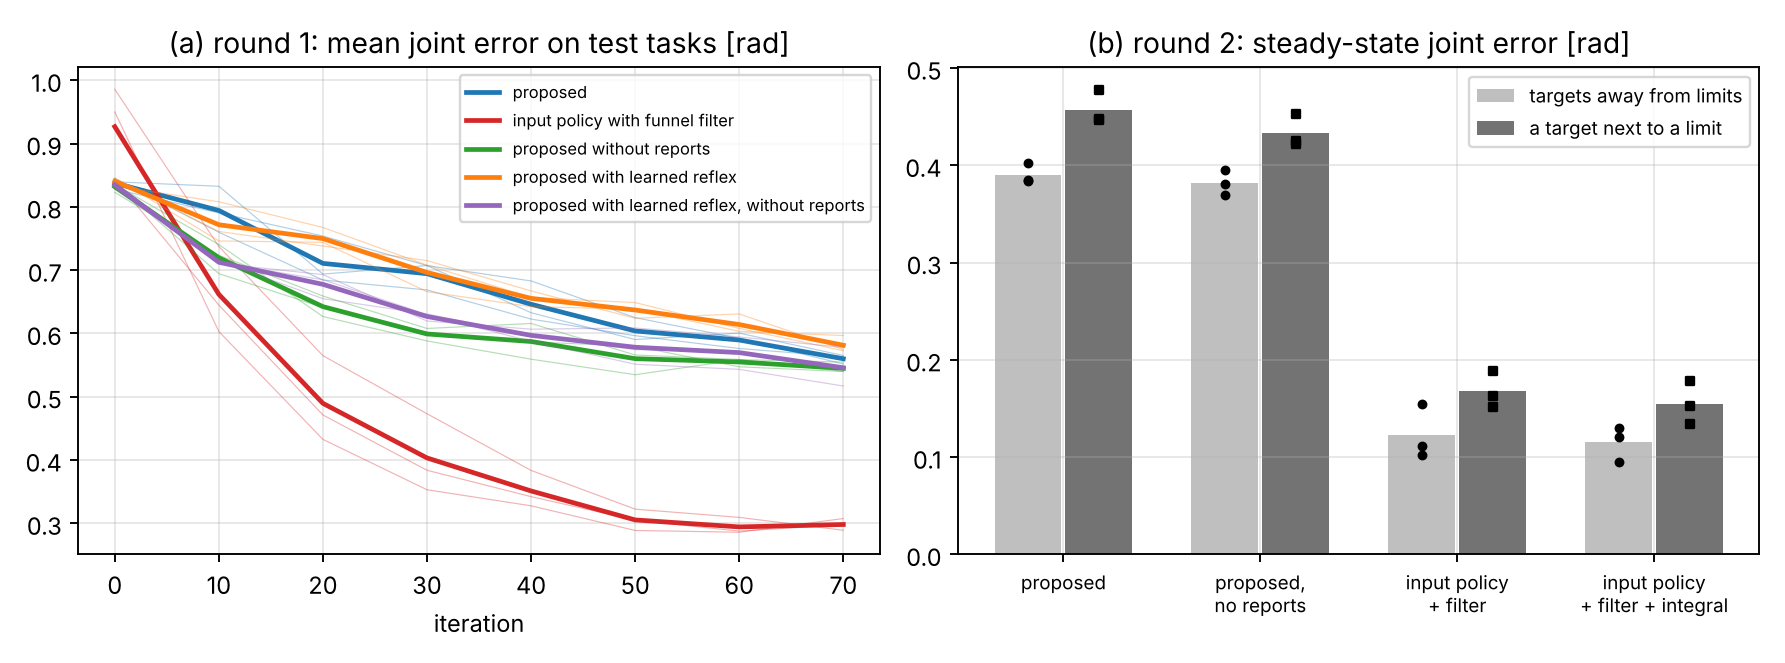
\includegraphics[width=0.98\textwidth]{rl_comparison.png}
\caption{Joint error of the learned policies in the two rounds}
\label{fig:rl}
\end{figure}

\Cref{fig:rl}(a)는 1차 비교의 학습 곡선(seed 평균과 개별 seed), (b)는 2차 비교의 정상 상태 오차를 목표 위치로 나눈 것이다.

\section{원인 확인: 사전 등록}
\label{sec:causes}

\textbf{직관 (진단을 하나씩 고친다).} 2차 비교 뒤의 분석은 제안한 구조가 뒤진 원인으로 네 가지를 들었다. 각 진단을 하나의 수리로 바꾸어 따로, 그리고 함께 시험했고, 판정 기준과 결과의 쓰임을 미리 기록했다. 기록 파일은 \texttt{records} 폴더의 \texttt{preregistration\_causes.md}이고, SHA-256의 앞 8자리는 \texttt{d158152c}이다. 나머지 설정은 1차 비교와 같다.
\begin{itemize}
\item[\textbf{(D1)}] 허용 오차 tube가 운동을 느린 reference에 묶는다. 수리: 허용 오차 상한을 0.4에서 1.0으로 올린다. 새 속도 상한 4.0 rad/s에서 drift 배율의 최솟값은 1.210이므로 정리가 계속 적용된다.
\item[\textbf{(D2)}] Feedback gain이 학습 밖에 있다. 수리: task policy가 $\kappa/\psi_g^2$를 $[15,60]$에서 고른다.
\item[\textbf{(D3)}] 속도형 action은 배우기 어렵고 양보가 그 효과를 지운다. 수리: task policy가 목표 위치를 내고, reference는 그쪽으로 비례 조향된다.
\item[\textbf{(D4)}] 적응 표현이 약하다. 수리: plant class의 표본에서 meta-learning한 feature 20개를 쓰고, 그 평균 task weight를 fast weight 초기값으로 둔다. 과제별 최소제곱의 상대 잔차는 $1.12\times10^{-4}$로 무작위 feature 29개의 $1.20\times10^{-2}$보다 약 100배 작다.
\end{itemize}
판정 기준은 다음과 같다. 수리 하나가 세 seed 모두에서 관절 오차를 1차 비교 대비 20\% 이상 줄이면 그 진단을 지지한다. 네 수리를 함께 켠 구조가 기존 방식과의 차이를 절반 이상 줄이면(seed마다 0.429 rad 이하) 허용 오차 계층을 다음 설계의 후보로 남기고, 그렇지 않으면 버린다.

\begin{table}[H]
\centering\footnotesize\setlength{\tabcolsep}{4pt}
\caption{Pre-registered cause check}
\label{tab:causes}
\begin{tabular}{p{3.3cm}ccccc}
\toprule
수리 & seed별 관절 오차 [rad] & 1차 비교 대비 [\%] & 판정 & yield factor 평균 & 위반 \\
\midrule
D1 looser tolerance & 0.542, 0.616, 0.532 & $-1.8$, $+9.4$, $-5.8$ & 기각 & 0.65 & 0 \\
D2 learned gain & 0.531, 0.488, 0.537 & $-3.8$, $-13.3$, $-4.9$ & 기각 & 0.65 & 0 \\
D3 target action & 0.565, 0.549, 0.566 & $+2.4$, $-2.4$, $+0.1$ & 기각 & 0.60 & 0 \\
D4 meta-learned features & 0.515, 0.479, 0.539 & $-6.6$, $-15.0$, $-4.7$ & 기각 & 0.89 & 0 \\
all four & 0.457, 0.455, 0.471 & $-17.2$, $-19.2$, $-16.7$ & 기각 & 0.84 & 0 \\
\bottomrule
\end{tabular}
\end{table}

네 진단은 모두 기각되었다. 단독 효과가 가장 큰 것은 feature 수리(평균 $-8.8\%$)였고, tolerance 상한 수리는 효과가 없었다(평균 $+0.6\%$). 미리 예측한 순서 가운데 (D4)가 가장 크다는 것은 맞았고 (D1)이 크다는 것은 틀렸다. 네 수리를 함께 켜면 오차는 0.455--0.471 rad로 줄었지만 기준 0.429 rad에 미치지 못했다(\Cref{fig:causes}). 위반은 모든 변형에서 없었다. 규칙에 따라 다음 설계에서는 허용 오차 계층을 버린다.

\begin{figure}[H]
\centering
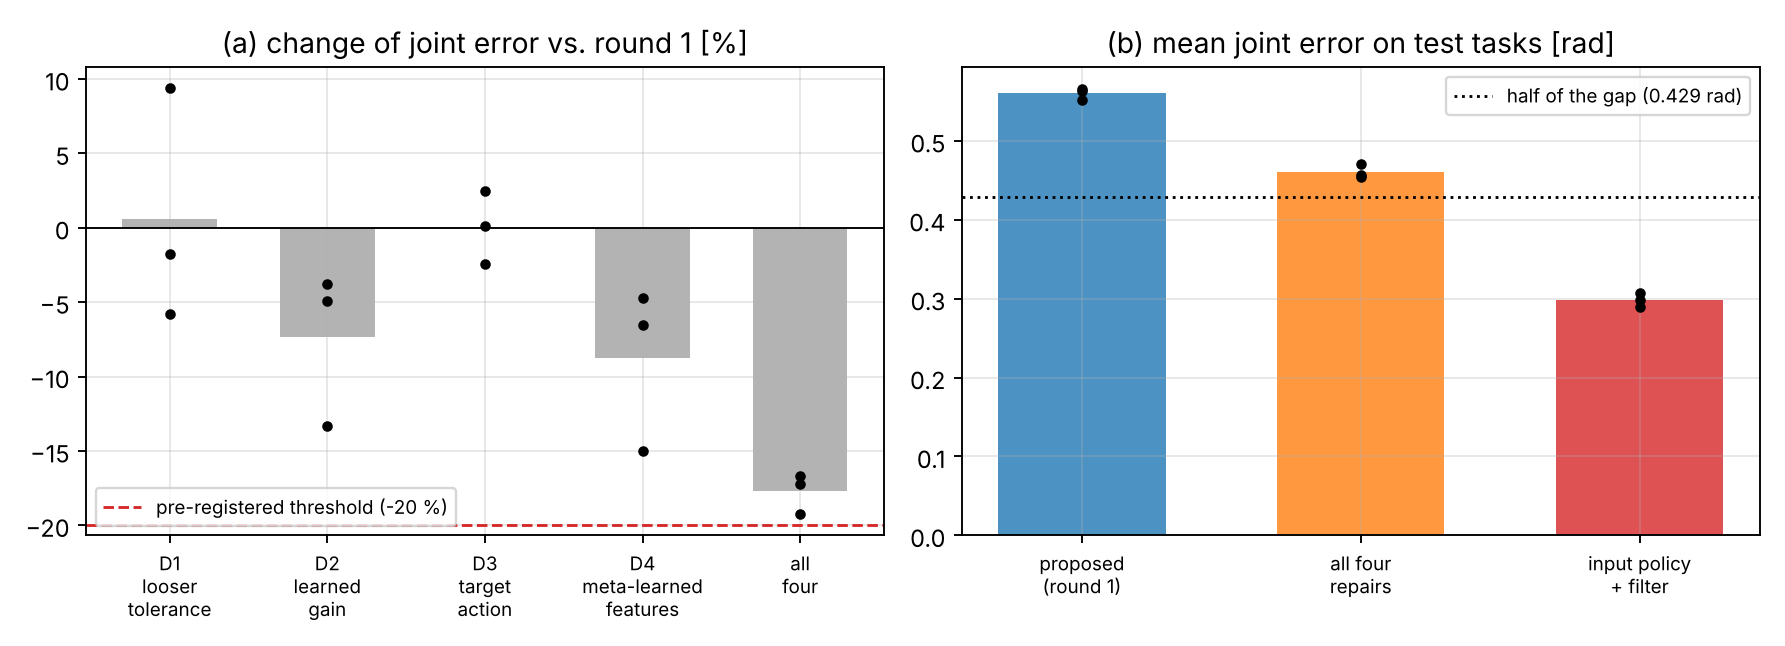
\includegraphics[width=0.98\textwidth]{cause_check.png}
\caption{Pre-registered cause check}
\label{fig:causes}
\end{figure}

\textbf{무엇이 남는가.} Feature 수리로 양보가 거의 사라졌는데도(yield factor 평균 0.83--0.94) 오차는 0.479--0.539 rad에 머물렀다. 따라서 양보는 주된 원인이 아니다. 운동학적 한계도 주된 원인이 아니다. Torque 한계, plant 동역학, clearance를 빼고 계층이 허용하는 운동만 남기면 문제는 다음과 같다.
\[
\eta=r_g+d,\qquad \norm{\dot r_g}\le\bar v,\qquad \norm{d}\le\psi_{\max},\qquad \dot q=\eta-k_1q .
\]
이 문제에서 test task 평균 오차가 0.190 rad인 운동이 존재한다($\bar v=4$, $\psi_{\max}=0.4$). 이 값은 볼록 문제에 projected gradient를 3,000번 적용한 결과이고 최적값은 이보다 작으며, 기존 방식의 0.298 rad보다 작다. 남는 설명으로 가장 가능성이 큰 것은 reference에서 actuator까지의 지연 사슬이다. Core의 추종 시간 상수 $\lambda_{\max}(M)/K_C\approx0.2$초와 위치 filter의 지연 $1/k_1=0.5$초가 겹치고, 이를 보상하려면 위층이 reference를 앞서 보내야 하는데 학습은 그 해를 찾지 못했다. 기존 방식은 actuator 수준에서 직접 행동하므로 이 사슬이 없다. 이 설명은 직접 시험하지 않았다.

\section{선행 연구와의 대조}
\label{sec:lit}

\textbf{가장 가까운 선행 연구 (전문).} Das와 Jagtap은 모델을 모르는 Euler--Lagrange system에서 입력 한계 아래 funnel을 넓히지 않고 유지하며, 알려진 상한으로 실행 가능 조건을 명시한다. 7-DOF manipulator 실험도 포함한다. 따라서 실행 가능한 reference에 대해서는 고정된 오차 경계와 입력 한계를 함께 보장하는 명시적 조건이 이미 있다.

\textbf{결합된 관성.} 그들의 조건은 성분별이다. 증명의 둘째 단계는 한 성분의 입력이 한계에 있을 때 그 성분의 가속도를 Assumption 3으로 누르는데, 그 가정은 입력 한계 벡터의 한 부호 조합에 관한 것이다. 다음 행렬에서 그 가정은 $\underline m=6.125$로 성립한다.
\[
M^{-1}=5\begin{pmatrix}1&0.9\\0.9&1\end{pmatrix},\qquad \bar\tau=(2,8),\qquad M^{-1}\bar\tau=(46,49).
\]
그러나 부호가 섞인 입력에서는 해당 가속도 성분의 부호가 증명이 쓰는 값과 반대이다.
\[
\tau=(-2,8)\ \Longrightarrow\ (M^{-1}\tau)_1=26>-\underline m\,\bar\tau_1=-12.25 .
\]
강하게 결합된 관성에서는 그 논증이 이 경우를 다루지 않는 것으로 보인다. 이 행렬이 실제 manipulator에서 나오는지는 확인하지 않았다. 제약 노트의 방향별 조건은 이 경우를 포함하지만, 그 차이는 기술적 보완이다.

\textbf{그 밖의 결과.} Ni 등은 결합된 입력의 MIMO system에서 saturation이 작동할 때 성능 경계를 넓히고 끝나면 좁히는 방식을 제시한다(전문). 그들은 plant가 bounded-input bounded-state 안정이라고 가정하고, 그렇지 않은 결합 system의 실행 가능 조건을 미해결로 남긴다. Reference 수정 방식의 원 논문과 성분별 수정 방식들은 공개 전문을 찾지 못해 Ni 등의 서술로만 확인했다. Funnel 제어를 학습 중의 안전장치로 쓰는 연구도 있다(초록).

\section{결론}
\label{sec:concl}

제안한 구조는 증명대로 제약을 지켰지만, 같은 예산의 학습에서 기존 방식보다 나빴고 기존 방식도 이 과제에서 제약을 지켰다. 보고는 return을 높이지 않았고, 사전에 등록한 예측도 기각되었다. 이론 결과 가운데 실행 가능한 reference에 대한 부분은 선행 연구에 있다. 따라서 이 설계는 중단한다.

\textbf{원인 확인의 결론.} 미리 지목한 네 원인 가운데 단독으로 기준을 넘은 것은 없었고, 가장 유력하다고 본 tolerance tube 가설은 지지되지 않았다. 네 수리를 합쳐도 기존 방식과의 차이를 절반도 줄이지 못했으므로, 다음 설계는 허용 오차 계층 없이 actuator 수준에서 학습하는 적응형 controller와 경계에서만 개입하는 제약층으로 간다.

\textbf{남는 것.} 제약 노트의 정리들, 즉 방향별 authority 아래의 제약 보장, 기계 system으로의 축소, 관성 행렬을 모르는 경우의 storage 감소는 증명된 결과로 남는다. 임의의 명령에 대해 보장을 유지한다는 차이도 남지만, 이 비교에서 그 차이는 성능 이득으로 이어지지 않았다.

\textbf{범위.} 결론은 한 과제, 한 학습 알고리즘(70 iteration의 evolution strategies), seed 3개에 대한 것이다. 더 긴 학습, 다른 알고리즘, 다른 과제에서의 결과는 알지 못한다.

\appendix

\section{참고문헌과 확인 범위}
\label{app:refs}

\textbf{전문을 읽음.}
\begin{itemize}
\item R. Das, P. Jagtap, ``Prescribed performance control of unknown Euler--Lagrange systems under input constraints,'' arXiv:2507.01426v2.
\item J. Ni, X. Huang, G.~A. Rovithakis, Y. Yan, ``Low-complexity control under input saturation and performance constraints: a bidirectional modification scheme,'' arXiv:2609.00827.
\end{itemize}

\textbf{초록 또는 다른 논문의 서술만 확인함.}
\begin{itemize}
\item F. Fotiadis, G.~A. Rovithakis, ``Input-constrained prescribed performance control for high-order MIMO uncertain nonlinear systems via reference modification,'' IEEE Transactions on Automatic Control 69(5):3301--3308, 2024.
\item P.~S. Trakas, C.~P. Bechlioulis, ``Adaptive performance control for input constrained MIMO nonlinear systems,'' IEEE Transactions on Systems, Man, and Cybernetics: Systems 54(12):7733--7745, 2024.
\item T. Tao, C.~P. Bechlioulis, D.~V. Dimarogonas, ``Distributed adaptive prescribed performance control for interconnected Euler--Lagrange systems under input constraints,'' IEEE Transactions on Control of Network Systems 12(4):2932--2943, 2025.
\item L. Lanza, D. Dennst\"adt, K. Worthmann, P. Schmitz, G.~D. \c{S}en, S. Trenn, M. Schaller, ``Sampled-data funnel control and its use for safe continual learning,'' arXiv:2303.00523.
\end{itemize}

\textbf{알려진 것, 다시 열어 보지 않음.} T. Salimans, J. Ho, X. Chen, S. Sidor, I. Sutskever, ``Evolution strategies as a scalable alternative to reinforcement learning,'' arXiv:1703.03864, 2017.

\end{document}
